\documentclass[preprint,11pt,authoryear]{elsarticle}
\usepackage{amsmath,amsthm}
\usepackage{newtxtext,newtxmath}
\usepackage{graphicx,booktabs}
\usepackage{microtype}
\usepackage[colorlinks,citecolor=teal,linkcolor=teal,urlcolor=teal]{hyperref}

\theoremstyle{remark}
\newtheorem{remark}{Remark}

% elsarticle prints "Preprint submitted to ..." on the title page; suppress it.
\makeatletter
\def\ps@pprintTitle{%
  \let\@oddhead\@empty\let\@evenhead\@empty
  \let\@oddfoot\@empty\let\@evenfoot\@oddfoot}
\makeatother

\begin{document}

\begin{frontmatter}

\title{Locating community thresholds along contamination gradients with Euler
characteristic surfaces}

\author[gwu]{Sushovan Majhi\corref{cor}}
\ead{s.majhi@gwu.edu}
\cortext[cor]{Corresponding author.}
\author[mtu]{Robert Pal}
\author[mtu]{Atish Mitra}
\author[rf]{Ying Sun}

\affiliation[gwu]{organization={George Washington University},
  city={Washington, DC}, country={USA}}
\affiliation[mtu]{organization={Montana Technological University},
  city={Butte, MT}, country={USA}}
\affiliation[rf]{organization={Rare Flora, Inc.}, country={USA}}

\begin{abstract}
Whether degraded plant communities respond to contamination smoothly or at
thresholds decides where remediation effort pays. The standard tools---threshold indicator taxa analysis (TITAN), gradient forest, breakpoints on
ordination axes---assemble a community threshold from taxon-level abundance
change, and so cannot see a community whose taxa rearrange their co-occurrence
structure while each abundance profile stays put. We summarize co-occurrence
structure within sliding windows of plots by the Euler characteristic of a
flag complex, indexed by edge count so that connectance is fixed and only
arrangement varies, and locate the change with a pooled two-sample split, a
plot-permutation test, and a within-window bootstrap. The indexing is
essential: under a similarity-indexed filtration, edge density alone separates
simulated communities more strongly than the Euler characteristic does.
Fixed on simulated gradients before any field data were analyzed, the
estimator recovers a known threshold (RMSE 0.10 of gradient span at 160
plots), holds false-positive rates near nominal, and gains power with plots
(0.18 at 80, 0.66 at 160) or with repeat surveys stacked into windows. It
and TITAN each miss the other's signal: pure abundance shifts versus
co-occurrence reorganizations. On TITAN's
Everglades benchmark the frozen estimator places the change at 12.5~$\upmu$g/L
total phosphorus, near TITAN's decliner change point and the 10~$\upmu$g/L
water-quality criterion, but the permutation test does not reject
($p = 0.30$), as the power analysis predicts at 126 sites. We state the
analysis protocol for a Superfund restoration network before its data are
seen, and release Python and R implementations.
\end{abstract}

\begin{keyword}
ecological thresholds \sep co-occurrence networks \sep Euler characteristic
\sep topological data analysis \sep mine-land reclamation \sep
pre-registration
\end{keyword}

\end{frontmatter}

\section{Introduction}
\label{sec:intro}

Reclamation of metal-contaminated land is judged against targets that presume a
response shape. If plant community structure degrades smoothly with soil metal
load, then any reduction in contamination buys a proportionate improvement and
targets can be set anywhere on the gradient. If instead the community reorganizes
at a threshold, then effort spent on the wrong side of that threshold buys very
little, and effort that crosses it buys a great deal. The distinction is
practical before it is theoretical
\citep{groffman2006thresholds}, and on a Superfund landscape it decides where
remediation dollars go.

Detecting such thresholds from community data is well studied. The dominant
approach, Threshold Indicator Taxa Analysis \citep[TITAN;][]{baker2010titan},
scores each taxon's change in abundance and occurrence across every binary
partition of the gradient, building on indicator species analysis
\citep{dufrene1997indval}, then aggregates the taxon-level change points into a
community-level threshold. TITAN is deservedly standard: it is interpretable,
it names the taxa driving the signal, and it has a careful treatment of
uncertainty \citep{king2010titan2}. Its structure also fixes what it can see.
Because the community threshold is assembled from taxon-level scores, a
reorganization that changes how taxa are arranged relative to one another
without shifting individual abundance--occurrence profiles is not, by
construction, what the statistic is built to detect. The method's own authors
have written at length on where it is misapplied \citep{baker2013limits}.

The same observation covers the rest of the standard toolkit. Breakpoint
regression locates a threshold in a chosen univariate response, classically an
ordination axis \citep{toms2003piecewise}, so it sees what the ordination
preserves---dominant compositional turnover---and inherits the ordination's
indifference to how taxa covary around that turnover. Gradient forest
\citep{ellis2012gradientforest} aggregates split importances of taxon-level
response functions, one taxon at a time, and so is taxon-aggregative in the
same sense TITAN is. None of these methods is wrong; they are instruments
pointed at taxon-level change. The blind spot they share is a community whose
taxa keep their individual gradient profiles while rearranging their joint
structure---who co-occurs with whom, and how tightly. The summary-free
statistical route---nonparametric multivariate change-point detection on
the raw plot sequence, of which e-divisive is the standard instance
\citep{matteson2014ediv,james2015ecp}---covers distributional change in
principle, but energy statistics at survey-scale $n$ in taxon-space
dimension turn out to have essentially no power for changes that live in
the covariance structure, a claim Section~\ref{sec:swap} makes quantitative
rather than asserts. Section~\ref{sec:titan}
makes the gap concrete in both directions: on a simulated gradient whose
correlation structure reorganizes while every marginal abundance distribution
is held fixed, TITAN returns a handful of scattered, noise-level flags whose
change points spread across the gradient---no coherent community threshold---while on the converse simulation, an abundance shift with fixed
correlation structure, its indicator taxa recover the threshold
(Section~\ref{sec:titan} reports both instruments on both gradients).

Joint structure is not unstudied territory in ecology---co-occurrence
network analysis is an established practice, particularly in microbial
ecology, where network properties are routinely compared across conditions
and stress gradients \citep{barberan2012networks,faust2012microbial,
devries2018networks}. That literature is where the present method's substrate
comes from, and also where its cautionary tale lives: the network summaries
in common use---connectance, mean degree, modularity computed on graphs
thresholded at a fixed similarity---are exposed to the density confound
demonstrated in Section~\ref{sec:simfail}, and comparisons across conditions
are typically descriptive, without an estimator or a significance framework
for \emph{where} along a gradient the structure changes. What we add to that
practice is the connectance control, an explicit localization estimator with
pre-registered inference, and the demonstration of when a topological summary
carries signal that the similarity distribution itself does not
(Section~\ref{sec:swap}).

We take a different route to the same question. Rather than aggregating
taxon-level responses, we summarize the \emph{shape} of the community's
co-occurrence structure with a single integer---its Euler characteristic---and ask where along the gradient that shape changes. The Euler characteristic is
cheap, requires no ordination or distributional assumption, and is stable under
perturbation of the underlying data \citep{dlotko2023eulercurves}. It has been
used to summarize time series \citep{sharma2026ecs}, to give regime transition
in a dynamical system a mathematical definition \citep{majhi2026regime}, and, in
the application that motivates the present construction, to locate the
slug/churn transition in multiphase pipe flow and correct a
forty-year-old industry-standard flow-regime map from thirty-seven trials
\citep{koenig2026churn}. Locating a transition along an ordered parameter is the
same problem in each case; only the substrate differs. One boundary is worth
drawing before any construction is given: the instrument answers \emph{where}
along the gradient the community's joint structure changes fastest, and
whether that change is gradient-associated at all. Whether the change is a
discontinuity in the strict sense---the threshold-versus-smooth dichotomy
of the opening paragraph---turns out, in our own calibration, to demand
more data than the survey designs we study can supply
(Section~\ref{sec:power}), and we are explicit throughout about that limit.

Two things make the transfer non-trivial, and both are reported here because
neither is obvious in advance.

First, \textbf{the naive construction measures connectance, not shape}. If the
Euler characteristic is computed on a thresholded co-occurrence \emph{graph},
then $\chi = V - E$ identically, so the resulting curve is a reparametrization
of the number of edges present and carries no topological information at all.
The summary must be taken on a complex of dimension at least two.

Second, and less obviously, \textbf{even the higher-dimensional summary is
dominated by connectance if the filtration is indexed by similarity}. In
simulation (Section~\ref{sec:sim}) a plain edge-density curve separated two
communities better than the Euler characteristic did, and the topological
signal proved to be the density signal in another coordinate. The remedy is to
index the filtration by the number of edges admitted rather than by a similarity
threshold, which holds connectance fixed by construction and leaves only
structure. Comparing networks at matched density is long-standing practice in
network neuroscience for exactly this reason
\citep{achard2006resilient,vanwijk2010density}; to our knowledge it has not been
combined with an Euler characteristic filtration, nor applied to community
ecology.

This paper contributes, in order: (i) the demonstration that similarity-indexed
topological summaries of co-occurrence structure are connectance measurements in
disguise, and the connectance-controlled construction that repairs them
(Sections~\ref{sec:complex}--\ref{sec:connectance}, \ref{sec:simfail});
(ii) a threshold estimator on the resulting Euler characteristic surface---window rule, change statistic, bootstrap interval, and permutation test---selected on simulated gradients with known thresholds and stated precisely
enough to be pre-registered, which it is, here, before any field data was seen
(Section~\ref{sec:est}); (iii) a simulation study giving the estimator's
recovery error, its power as a function of survey design---including what
repeat annual surveys buy, and how they must be used to buy it---and a
negative result on a proposed sharpness diagnostic
(Sections~\ref{sec:simgrad}, \ref{sec:power}); (iv) evidence that the method and taxon-aggregative detection
are complementary in both directions (Section~\ref{sec:titan}); (v) a real-data application on the incumbent's own
benchmark dataset, reported under the frozen protocol, alongside an
accounting of two public omics datasets that structurally cannot test the
central claim (Section~\ref{sec:public});
and (vi) the pre-registered analysis protocol for the Butte Hill restoration
network (Section~\ref{sec:butte}).

\section{Materials and Methods}

\subsection{Data and notation}
\label{sec:data}

Let $X \in \mathbb{R}_{\ge 0}^{S \times P}$ record the abundance of $S$ taxa
across $P$ plots, and let $z \in \mathbb{R}^{P}$ give each plot's position on the
environmental gradient---here soil metal concentration. Write $X_{\cdot A}$ for
the submatrix on a plot subset $A$. Everything below is agnostic to the survey's
specifics; the design guidance in Section~\ref{sec:power} says what $P$ buys.

\subsection{From abundance to a filtered complex}
\label{sec:complex}

Each taxon is represented by its abundance profile across the plots in $A$,
giving a point cloud of $S$ points in $\mathbb{R}^{|A|}$. We use correlation
distance
\[
  d(i,j) \;=\; 1 - \mathrm{corr}\!\left(X_{i A},\, X_{j A}\right)
  \;\in\; [0,2],
\]
which is invariant to each taxon's overall abundance and therefore comparable
across plot subsets of differing productivity. A taxon with no variation
within $A$ (typically, absent from every plot in it) has undefined
correlation; it is assigned distance $1$ to every other taxon, so that it
enters the filtration only after all positively correlated pairs.

For a threshold $r$ let $G(r)$ be the graph on the $S$ taxa with an edge wherever
$d(i,j) \le r$, and let $K(r)$ be its flag complex: the simplicial complex whose
$k$-simplices are the $(k+1)$-cliques of $G(r)$. The Euler characteristic is the
alternating sum of simplex counts,
\[
  \chi\bigl(K(r)\bigr) \;=\; \sum_{k \ge 0} (-1)^{k}\,
  \bigl|\{(k{+}1)\text{-cliques of } G(r)\}\bigr|
  \;=\; V - E + T - \cdots .
\]

\begin{remark}
Truncating at $k \le 1$---that is, taking the graph itself rather than its
flag complex---gives $\chi = V - E$, which for fixed $S$ is an affine
function of the edge count. Any apparent signal in such a curve is
connectance and nothing else. Throughout we compute $\chi$ of the
$3$-skeleton of the flag complex (cliques of at most four taxa). Toward the
dense end of the edge-count grid larger cliques exist, so the quantity is the
Euler characteristic of the truncated complex rather than of the full flag
complex; the $3$-skeleta still form a filtration, and the summary is used
only comparatively, at identical truncation, across windows.
\end{remark}

\subsection{Indexing by connectance}
\label{sec:connectance}

Rather than evaluating $\chi$ on a fixed grid of thresholds $r$, we evaluate it
at a fixed grid of \emph{edge counts}. For a target count $m$, let $r(m)$ be the
$m$-th smallest pairwise distance,\footnote{The released code indexes
distances from zero, so its grid point $m$ admits $m+1$ edges; the fixed
offset of one edge is immaterial and is retained for exact
reproducibility.} and define
\[
  \chi_A(m) \;=\; \chi\bigl(K(r(m))\bigr).
\]
Because $G(r(m))$ has $m$ edges (up to ties) for every plot subset $A$, any difference
between $\chi_A(m)$ and $\chi_B(m)$ is a difference in how those $m$ edges are
arranged, not in how many there are. This is the single design decision on which
the method depends, and Section~\ref{sec:simfail} shows what happens without it.
Throughout we use twelve evenly spaced edge counts running from $2S/3$ to
approximately half of all $\binom{S}{2}$ pairs; the released code
(Section~\ref{sec:avail}) is definitive for the protocol. The grid density
is immaterial: because $\chi(m)$ is a cumulative sum and hence smooth in
$m$, halving or doubling the grid (6 or 24 points) leaves the simulated
recovery and the Everglades point estimate unchanged
(\texttt{results/14\_grid\_sensitivity.txt}).

\subsection{The surface and the pre-registered threshold estimator}
\label{sec:est}

Sliding a window along the gradient $z$ and stacking the resulting curves gives
\[
  \mathcal{E}(m, z) \;=\; \chi_{A(z)}(m),
  \qquad A(z) = \{\,p : z_p \in \text{window at } z\,\},
\]
the Euler characteristic surface over connectance and gradient position. A
threshold is a location where this surface changes fastest along $z$.

The estimator is fixed as follows, every choice having been made on the
simulated gradients of Section~\ref{sec:simgrad}---where the true threshold is
known---and none on field data.

\begin{enumerate}
\item \emph{Windows.} Order the plots by $z$. Windows contain
$W = \max(6, \mathrm{round}(P/4))$ consecutive plots and slide by
$\mathrm{round}(W/3)$, each window placed at the mean $z$ of its plots. The
window curves $\chi_{A_1}(\cdot), \dots, \chi_{A_K}(\cdot)$ evaluated on the
common edge-count grid are the data for everything below.
\item \emph{Change statistic and location.} For each candidate split $s$ with at
least two windows on each side, compute the absolute Cohen's $d$ between the
two groups of curves separately at each edge count, and average over the grid:
\[
  D(s) \;=\; \frac{1}{|\mathcal M|}\sum_{m \in \mathcal M}
  \bigl|\,d\bigl(\{\chi_{A_k}(m)\}_{k \le s},\,
               \{\chi_{A_k}(m)\}_{k > s}\bigr)\bigr| .
\]
The threshold estimate $\hat z$ is the midpoint of the window positions
flanking the maximizing split, and $D^\ast = \max_s D(s)$ is the test
statistic. Averaging over the grid, rather than maximizing, is what
stabilizes the location (Section~\ref{sec:simgrad}); maximizing over $m$
inflates small-sample noise, the failure mode documented on real data in
Section~\ref{sec:public}.
\item \emph{Significance.} Permute the plot positions along $z$, rebuild the
windows, and recompute $D^\ast$; with $B = 999$ permutations the $p$-value is
$(1 + \#\{D^\ast_b \ge D^\ast\})/(1+B)$. The permutation destroys the
association between community structure and gradient position while preserving
the window geometry and the connectance control, so this is a test of
\emph{association}, not of sharpness: a smooth structural trend will also
reject, as it should.
\item \emph{Uncertainty.} Resample plots with replacement within
each window, recompute the curves, and re-estimate $\hat z$; the 2.5--97.5
percentile interval over $999$ resamples is the confidence statement. We
attempted to calibrate the \emph{width} of this interval as a sharpness
diagnostic---the hope being that it concentrates on sharp thresholds and
stays wide under smooth change of the same magnitude---and the calibration
failed at survey scale: the widths are indistinguishable at $P \le 80$ and
only begin to separate at $P = 160$ (Section~\ref{sec:power}). The interval is therefore an uncertainty statement
only, and the method offers no test of thresholdness; $\hat z$ locates the
fastest structural change whether or not that change is discontinuous.
\end{enumerate}

The resolution of $\hat z$ is bounded by the window width: with windows
covering a quarter of the gradient, structure inside $\pm W/2$ of the true
threshold is mixed by construction, and the simulations bear this out---recovery error tracks window width, not the choice of statistic. Surveys
wanting sharper localization need more plots, not a cleverer estimator.

\section{Simulation study}
\label{sec:sim}

\subsection{Indexing by similarity fails}
\label{sec:simfail}

Two groups of communities were simulated---120 taxa in eight modules, fifteen
replicate communities per group---differing in how coherently the modules
respond across conditions. Sweeping a fixed similarity grid, edge density alone
separated the two groups at $\max|\mathrm{Cohen}\ d| = 4.59$, against $2.20$
for $\chi$ of the flag complex. Subtracting the Erd\H{o}s--R\'enyi expectation
of $\chi$ at the observed edge count---a density-matched null---left the
separation at $2.21$: under a similarity sweep the topological summary carries
no separation beyond what connectance already supplies.

\subsection{Indexing by connectance isolates structure}

At matched edge counts the comparison inverts. Two point configurations in
$\mathbb{R}^3$ (Euclidean distance; 120 points, fifteen replicates each)---eight modules placed independently, and the same modules arranged on a cycle---have identical connectance at every grid point by construction, and the
connectance-indexed $\chi$ separated them at
$\max|\mathrm{Cohen}\ d| = 4.71$ (Figure~\ref{fig:confound}). Once
connectance is controlled, the summary responds to arrangement. Whether it
also carries information that the distance distribution does not is a
separate question, taken up in Section~\ref{sec:swap}.

\begin{figure}[t]
\centering
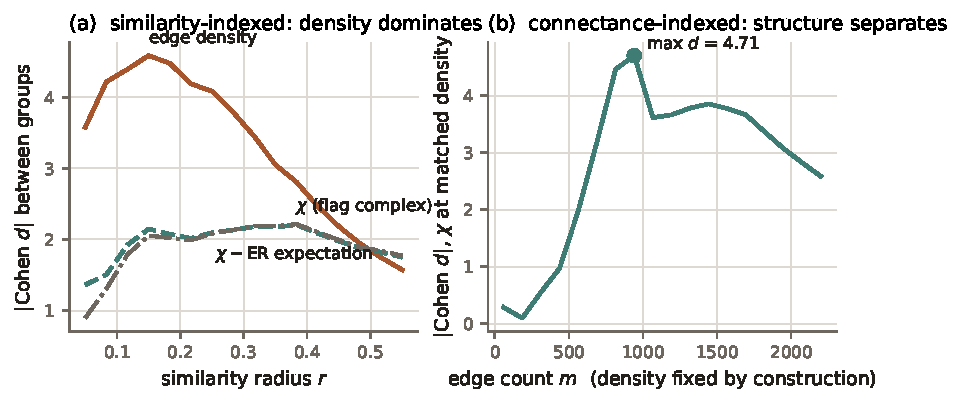
\includegraphics[width=\textwidth]{figs/fig1_confound.pdf}
\caption{The confound and the fix. (a) Under a similarity-indexed sweep,
plain edge density separates the two simulated communities better than the
Euler characteristic, and subtracting the density-matched
Erd\H{o}s--R\'enyi expectation from $\chi$ leaves the same curve---the topological summary is the connectance signal reprocessed.
(b) Indexing by edge count holds connectance fixed by construction, and two
configurations with identical density separate on arrangement alone.}
\label{fig:confound}
\end{figure}

\subsection{Simulated gradients, and the choice of estimator}
\label{sec:simgrad}

To fix the estimator we simulated gradients with a known threshold. Sixty taxa
in six modules load on latent factors ($\rho = 0.55$); above the threshold
$z^\ast = 0.55$, paired modules begin sharing a factor with mixing weight
$0.7$, so the community reorganizes from six blocks into three super-blocks.
Critically, every taxon's marginal abundance distribution is identical at every
gradient position---unit variance throughout, by construction---so the
gradient carries \emph{only} co-occurrence reorganization, the signal the
methods of Section~\ref{sec:intro} are not built to see. Plots are placed uniformly at
random on the gradient; designs of $P = 40$, $80$, and $160$ plots use the
window rule of Section~\ref{sec:est}.

Three change statistics were candidates: the discrete derivative of the surface
along $z$; the two-sample split, with $|d|$ either maximized or averaged over
the edge-count grid; and a two-segment continuous fit with the break location
shared across the grid. Table~\ref{tab:est} reports recovery of $z^\ast$ over
100 realizations per design, and the mean statistic on threshold,
smooth-change, and no-change gradients.

\begin{table}[t]
\centering
\caption{Estimator selection on simulated gradients (true $z^\ast = 0.55$;
gradient span $[0,1]$; 100 realizations per design). RMSE of $\hat z$ on
sharp thresholds; mean statistic on threshold (T), smooth (S), and null (N)
gradients at $P=80$. Bias is below $0.05$ for every candidate at every size.
The pooled split is the only candidate whose statistic ordering
$\mathrm{T} \ge \mathrm{S} \ge \mathrm{N}$ holds at all three design
sizes; the derivative is dominated by small-sample noise, the maximized
split loses the ordering at $P = 40$, and the fitted break barely separates
signal from null.}
\label{tab:est}
\begin{tabular}{lcccccc}
\toprule
 & \multicolumn{3}{c}{RMSE of $\hat z$}
 & \multicolumn{3}{c}{statistic at $P=80$} \\
\cmidrule(lr){2-4}\cmidrule(lr){5-7}
Statistic & $P=40$ & $P=80$ & $P=160$ & T & S & N \\
\midrule
derivative along $z$        & 0.228 & 0.226 & 0.218 & 3.16 & 3.10 & 3.13 \\
split, $\max_m |d|$          & 0.204 & 0.170 & 0.120 & 4.85 & 3.83 & 3.32 \\
two-segment fit             & 0.204 & 0.184 & 0.161 & 0.30 & 0.31 & 0.30 \\
\textbf{split, mean over $m$} & 0.203 & \textbf{0.160} & \textbf{0.103}
                            & 2.15 & 1.78 & 1.51 \\
\bottomrule
\end{tabular}
\end{table}

The pooled split has the best recovery at the two larger designs and is the
only statistic whose signal-to-null ordering holds everywhere---so it is
the estimator, fixed before any field data. Two observations
accompany it. At $P = 40$ the separation is marginal for every candidate
(the pooled split gives 1.59 against a null of 1.50), and detection at that
design size fails for reasons quantified next. And recovery error at every
size tracks half the window width, confirming that localization is
resolution-limited, not statistic-limited.

\subsection{Power, false positives, and sharpness}
\label{sec:power}

This section turns the switchgrass failure of Section~\ref{sec:public} into
design guidance: the question a survey must answer in advance is what plot
count per window resolves an effect worth caring about. We report the
permutation test's rejection rate on sharp-threshold gradients and its false
positive rate on no-change gradients at three design sizes, and the bootstrap
calibration promised in Section~\ref{sec:est}.

At $\alpha = 0.05$ with 499 permutations of plot positions and 50
realizations per cell, the test rejected sharp-threshold gradients at rates
$0.00$, $0.08$, $0.18$, and $0.66$ for $P = 24$, $40$, $80$, and $160$, with
false-positive rates on no-change gradients of $0.08$, $0.02$, $0.02$, and
$0.06$, and rejected the abundance-shift gradient in $0.00$ of runs at
$P = 80$ and $0.04$ at $P = 160$. Three readings. False-positive rates lie
within Monte Carlo error of the nominal level at every size (the standard
error of a rate near $0.05$ is about $0.03$ at 50 realizations), and the
selectivity is as designed.
The absolute power at single-survey scale is modest---roughly a fifth of
strong reorganizations detected at 80 plots---and is reported as a design
constraint: precisely the switchgrass lesson. And power is
bought with plots per window---$0.66$ at $P = 160$---which motivates the
two extensions below, because a monitoring network does not need more land
to reach that regime; it needs its repeat surveys used correctly
(Figure~\ref{fig:design}).

\begin{figure}[t]
\centering
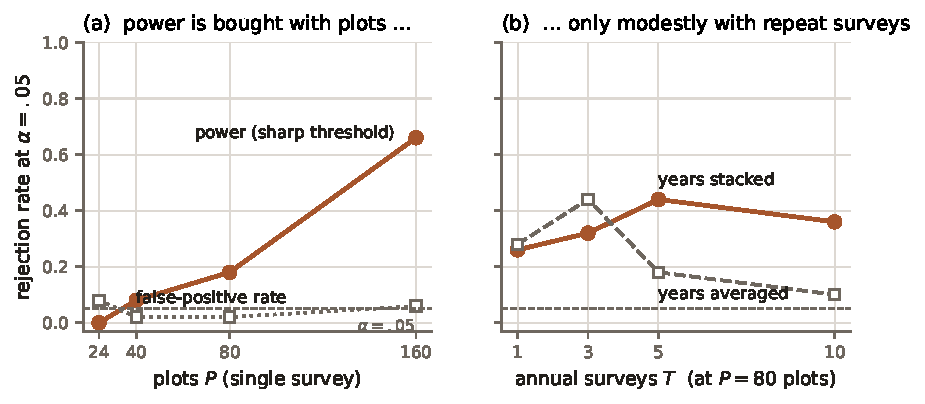
\includegraphics[width=\textwidth]{figs/fig2_design.pdf}
\caption{Design guidance. (a) Power against single-survey plot count
(499 permutations, 50 realizations per cell); false-positive rates stay at
the nominal level. (b) At $P = 80$, repeat annual surveys restore power only
when plot-years are \emph{stacked} as additional window columns (the
permutation moves whole plots); averaging years per plot cleans the wrong
noise term and buys nothing (99 permutations, 15 realizations per cell).}
\label{fig:design}
\end{figure}

Three further design results follow. First, coverage: the 95\% bootstrap
percentile interval contained the true threshold in 20 of 20 realizations at
$P = 80$ (mean width 0.49 of gradient span)---the interval is conservative,
erring wide rather than narrow, consistent with the resolution limit rather
than with over-confidence.

Second, repeat surveys---the result that decides whether the
Section~\ref{sec:butte} protocol is a fair test. The Butte Hill network has
roughly 80 plots and has been monitored since 2015, so repeat surveys may
span up to a decade (the data inventory will confirm how many); we simulated communities
in which a fraction $\tau = 0.3$ of latent community variance is
year-specific and asked what $T$ repeat surveys buy. The answer depends
entirely on how they are used. \emph{Averaging} years within plots buys
nothing---power $0.33/0.33/0.27/0.27$ at $T = 1/3/5/10$---because
averaging cleans each plot's measurement while the binding noise is the
sampling variability of correlations across the $W$ plots in a window, which
it cannot touch. \emph{Stacking} plot-years as additional samples attacks
that term directly: windows carry $W \times T$ columns, the permutation
moves whole plots so that a plot's years stay together, and power roughly
doubles---$0.47$ at $T = 3$ and $0.73$ at $T = 5$, with false-positive
rates at or below $0.07$ throughout---before saturating ($0.53$ at
$T = 10$) as within-plot redundancy bounds the effective sample size. The
protocol therefore stacks years rather than averaging them, and a
Butte-scale design with five or more surveys sits in the regime where the
test has real power.

The sharpness calibration returned a negative at survey scale, with a first
sign of life beyond it. At $P = 80$ (50 realizations per cell, 200
resamples) the bootstrap interval width on sharp thresholds (mean $0.515$)
is indistinguishable from its width under smooth change of the same
magnitude (mean $0.516$): the width is dominated by the resolution limit of
Section~\ref{sec:est}, not by the shape of the underlying change. At
$P = 160$ a gap begins to open---mean $0.440$ against $0.484$, and, more
tellingly, sharp thresholds produce intervals as tight as $0.145$ while
smooth change never fell below $0.289$---so the diagnostic may become
usable at design sizes beyond typical surveys, but at the sizes this paper
addresses we report the interval as uncertainty only. A survey
hoping to \emph{classify} its gradient response as threshold-like or smooth
needs either substantially more plots than the designs studied here or a
different instrument; what the present method delivers at these sizes is the
location of fastest change and the evidence that structure is
gradient-associated at all.

\subsection{The summary is modular---and when topology is necessary}
\label{sec:swap}

Nothing in the estimator of Section~\ref{sec:est} is specific to the Euler
characteristic: it consumes any curve-valued summary evaluated on the
connectance grid. We therefore ran six summaries through the same windows,
split, and permutation scheme---$\chi$ of the flag complex; the Betti curves
$\beta_0$ and $\beta_1$; greedy modularity of the $m$-edge graph, the summary
community ecology would reach for first; and two pure
correlation-distribution summaries, the distance quantile $r(m)$ and the mean
pairwise distance, which together are the concrete form of the objection
``why not just report the correlation distribution?''

The comparison needs gradient types that pull these apart. In the merge
scenario of Section~\ref{sec:simgrad} the correlation distribution and the
arrangement change together, so everything detects and nothing is learned
about attribution. We add two scenarios on a fixed module graph of six
modules, each carrying exactly two cross-module links of equal weight: a
\emph{rewiring} gradient, where the module graph switches from two triangles
to one hexagon at $z^\ast$---the degree structure and hence the expected
pairwise-correlation distribution are identical on both sides, only the
arrangement changes---and a \emph{strength} gradient, where the module
graph never changes but the cross-link weight halves at $z^\ast$, which
moves the correlation distribution while preserving the edge ranking and
therefore, at matched connectance, the complex itself. One wrinkle is
built in and reported: windows straddling $z^\ast$ mix
the two regimes, so a diluted transition signal leaks into distribution
summaries even on the rewiring gradient; the question the experiment answers
is how much signal each summary family retains where the other's is
designed away. These two scenarios use stronger coupling than
Section~\ref{sec:simgrad} (factor loading $\rho = 0.75$, mixing weight
$0.9$) so that cross-module links exceed the sampling noise of a window's
correlations. One adjustment to the statistic was needed for the comparison:
integer-valued Betti curves can have zero within-group variance, where
Cohen's $d$ is undefined, so each summary's curves are standardized and the
pooled within-group standard deviation is floored at $0.05$ of the
between-window standard deviation. The floor does not bind for $\chi$, whose
statistic is unchanged by it.

Table~\ref{tab:swap} reports the comparison at $P = 160$ over 100
realizations (statistics) and 50 realizations at 499 permutations
(rejection); at $P = 80$ no summary rejects any structured scenario at more
than $0.12$, consistent with Section~\ref{sec:power}. Three findings. On
the \emph{strength} gradient the designed asymmetry is confirmed: the
distance quantile rejects at $0.34$ while $\chi$ sits near its false-alarm
rate ($0.12$ against $0.06$)---matched-connectance summaries are blind to
distribution-only change, and distribution summaries see it, exactly as
constructed. On the \emph{rewiring} gradient the roles invert---but
weakly: the shape summaries' statistics separate from null ($\chi$ 1.74
against 1.38; modularity 1.97 against 1.46, rejecting at $0.18$ against
$0.02$) while the distance quantile stays below its null level (1.84
against 1.98), yet no summary clears $\alpha = 0.05$ reliably---arrangement-only reorganization is the hardest signal in this study, real
in the statistics and beyond dependable detection even at 160 single-survey
plots. And the transition-window leak declared above is visible: the mean
pairwise distance rejects rewiring at $0.14$ purely through the mixing of
regimes in straddling windows. On scenarios where detection occurs,
matched-connectance modularity is at least as strong as $\chi$ (merge
statistic $4.28$ against $3.13$; recovery RMSE $0.074$ against $0.102$)---a comparison we report rather than bury, because the framework is
summary-agnostic by design: $\chi$ is retained for its stability guarantee,
its deterministic clique-count computation, and its published
transition-localization lineage, not for empirical dominance over its
nearest shape-summary neighbor.

\begin{table}[t]
\centering
\caption{Six summaries through the identical pre-registered estimator at
$P = 160$ (true threshold $0.55$). Mean split statistic per scenario over
100 realizations, and permutation rejection at $\alpha = .05$ over 50
realizations with 499 permutations (in parentheses). REWIRE holds the
pairwise-correlation distribution fixed across the threshold; STRENGTH
moves the distribution while fixing the complex at matched connectance.}
\label{tab:swap}
\begin{tabular}{lccc}
\toprule
Summary & REWIRE & STRENGTH & no-change null \\
\midrule
$\chi$ (flag complex)   & 1.74 (.08) & 1.71 (.12) & 1.38 (.06) \\
$\beta_0$              & 2.11 (.14) & 2.10 (.08) & 1.91 (.08) \\
$\beta_1$              & 1.52 (.02) & 1.24 (.02) & 1.38 (.06) \\
modularity              & 1.97 (.18) & 2.23 (.14) & 1.46 (.02) \\
distance quantile $r(m)$ & 1.84 (.08) & 2.80 (.34) & 1.98 (.04) \\
mean pairwise distance  & 2.42 (.14) & 2.94 (.16) & 2.34 (.02) \\
\bottomrule
\end{tabular}
\end{table}

The summary-free statistical baseline completes the comparison. E-divisive
\citep{matteson2014ediv}, run on the raw ordered plot sequences themselves
(no windows, no summary; \texttt{ecp} with 199 permutations at
$\alpha = 0.05$), detected the merge gradient in 1 of 10 realizations at
$P = 80$---indistinguishable from its 1-in-10 false-alarm rate on the
matched null---and the rewiring gradient in 0 of 10 at both $P = 80$ and
$P = 160$---though Table~\ref{tab:swap} shows that even the shape
summaries, whose statistics do separate there, fall short of dependable
rejection on that hardest signal. This is
the expected behavior of energy statistics at survey-scale sample sizes in
taxon-space dimension: they are dominated by location alternatives, and a
change confined to the covariance structure starves them. The ecology
incumbents fare no better: PERMANOVA and PERMDISP
\citep{anderson2001permanova}, given the \emph{oracle} split at $z^\ast$---their best case, since neither localizes---rejected in 0--2 of 10 runs on
every scenario, signals and nulls alike (Euclidean distances, 199
permutations). Both test location and dispersion of sites in dissimilarity
space, and a reorganization that preserves every plot's marginal
distribution moves neither. The windowed, connectance-controlled summary is
not a convenience layer over standard multivariate testing; at these sizes
it is the difference between an instrument and none.

\subsection{Complementarity with taxon-aggregative detection}
\label{sec:titan}

The claim that the two instrument families see disjoint signals was tested in
both directions on the simulated gradients, five realizations each at $P=80$.
On \emph{reorganization} gradients (correlation structure changes at
$z^\ast$, all marginals fixed), TITAN---run with 250 permutations, 250
bootstrap replicates, purity and reliability cutoffs 0.95---flagged a median
of 4 of 60 taxa per run (range 1--9), with per-run median change points
scattered from 0.26 to 0.85 and \textit{sum(z)} intervals spanning most of the
gradient: background false flags at roughly the rate the cutoffs admit, and no
coherent community threshold. On \emph{abundance-shift} gradients (one
module's ten taxa shift mean abundance at $z^\ast$, correlation structure
fixed), it flagged 11--13 taxa per run, always including taxa of the shifted
module, with median indicator change points of 0.49--0.55 against a true
threshold of 0.55 in every run; the community-level sum($z+$) change point
fell at 0.53--0.56 in three of five runs and at 0.19 and 0.40 in the other
two.

\begin{table}[t]
\centering
\caption{Both instruments on both simulated gradient types ($P=80$, true
threshold 0.55). TITAN: five realizations per gradient type; $\chi$ split
test: 50 realizations, 499 permutations. Each responds to the signal it is
built for; the $\chi$ test's absolute power at this design size is limited
(Section~\ref{sec:power}), and its off-target rejection rate is zero.}
\label{tab:complement}
\begin{tabular}{lcc}
\toprule
 & reorganization gradient & abundance-shift gradient \\
\midrule
TITAN (pure \& reliable indicator taxa)
  & 1--9 of 60, scattered & 11--13 of 60, median cp at $z^\ast$ \\
$\chi$ split test (rejection at $\alpha=.05$) & 0.18 & 0.00 \\
\bottomrule
\end{tabular}
\end{table}

Neither result is a deficiency of either method; each is an instrument pointed
at a different component of community change. The practical recommendation
falls out directly: run both, and read disagreement as information about
\emph{which kind} of reorganization the gradient is driving. There is also
an ecological reason to want the covariance channel read at all: the
early-warning literature on critical transitions holds that changes in
correlation structure can \emph{precede} the abundance collapses that
taxon-level methods detect \citep{scheffer2009ews}---in which case a
structural threshold is a leading indicator, a boundary to act at before
species are lost rather than after. We note, without claiming it, that on
the Everglades data our point estimate falls on the early side of TITAN's
decliner change point (Section~\ref{sec:public}); whether that ordering is
real is exactly what an adequately powered design can test.

\section{Method validation on public gradients}
\label{sec:public}

\paragraph{A real ecological gradient: the Everglades phosphorus data.}
The demonstration an MEE reader will weigh most is on the incumbent's own
ground: the \texttt{glades} dataset shipped with TITAN2---126 marsh sites
by 164 macroinvertebrate taxa along a measured surface-water
total-phosphorus gradient, the demonstration data of \citet{baker2010titan}.
At $P = 126$ the window rule gives 32-site windows. The estimator is applied
as fixed on simulation before this dataset was first analyzed; preprocessing---taxa in at
least five sites, $\log(1+\text{abundance})$, gradient ordered by TP---was
fixed before outcomes were seen. One departure from Section~\ref{sec:est}:
for computational cost the test used 199 rather than 999 permutations and
the interval 199 bootstrap resamples; the Monte Carlo standard error of a
$p$-value near $0.3$ at 199 permutations is about $0.03$, immaterial to the
verdict.

The estimator places $\hat z = 12.5$~$\upmu$g/L TP, with a 95\% bootstrap
interval of $[12.0, 45.3]$. That point lies just below the 90\% bootstrap
interval of TITAN's decliner change point regenerated on the identical matrix
($15.1$, interval $13.2$--$19.9$; increasers $32.5$, interval $21.7$--$34.1$;
87 of 164 taxa pure and reliable) and just above the 10~$\upmu$g/L numeric
criterion that governs the system; our interval contains both of TITAN's
community change points.
But the permutation test does not reject ($p = 0.30$ over 199 permutations;
the distribution baseline $r(m)$ behaves similarly, $\hat z = 16.9$,
$p = 0.37$), and per protocol we therefore report \emph{no detection}. This
is the outcome the power analysis predicts rather than a surprise: 126
single-survey sites sit between the $P = 80$ and $P = 160$ rows of
Section~\ref{sec:power} (rejection $0.18$ and $0.66$ for a strong simulated
effect), so the run bounds the co-occurrence signal in these data rather
than refuting one. An exploratory run of the anchored secondary test of
Section~\ref{sec:butte} on these data---performed after the primary
result was seen, and labeled accordingly---also does not reject ($D = 0.99$
at the boundary nearest TITAN's decliner point, $p = 0.38$): the
non-detection is not merely the multiplicity cost of the free split. What
the run does establish, on the incumbent's own benchmark:
the frozen pipeline executes end to end at real survey scale, its point
estimate lands where the taxon-level evidence and the regulatory criterion
place the threshold region, and the verdict of a pre-registered test is
reported as such---the discipline Section~\ref{sec:butte} commits to for
Butte Hill, where stacked repeat surveys supply the power this
single-survey design lacks. Figure~\ref{fig:glades} shows the run
whole: the standardized window curves climb through the regulatory range,
crossing their mean almost exactly at $\hat z$.

\begin{figure}[t]
\centering
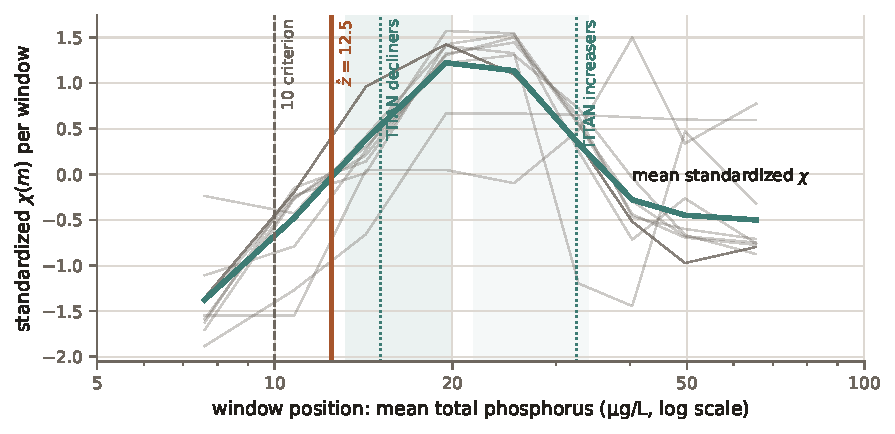
\includegraphics[width=\textwidth]{figs/fig3_glades.pdf}
\caption{The frozen estimator on the Everglades phosphorus gradient
(126 sites, 164 taxa; windows of 32 sites). Gray: standardized
$\chi(m)$ at each of the twelve edge counts, per window; the heavy line is
their mean. Vertical marks: the 10~$\upmu$g/L numeric criterion (dashed),
$\hat z = 12.5$ (solid), and TITAN's decliner and increaser change points
with their bootstrap intervals (dotted, shaded), regenerated on the
identical matrix. The permutation test does not reject ($p = 0.30$), and
the figure is reported as description, not detection.}
\label{fig:glades}
\end{figure}

\paragraph{Public omics data as stress tests.}
No public vegetation survey known to us pairs a plot network with a measured
contamination gradient at the scale Section~\ref{sec:butte} describes, so the
pipeline's remaining validation used two public transcriptomic datasets---the construction is agnostic to what the ``taxa'' are, and co-expression
gives it exactly the matrix shape of Section~\ref{sec:data} at realistic size and
noise. Both results bound what the pipeline can claim; neither supports it,
and we report them because the failure modes they exposed shaped the
estimator: the machinery runs end to end, the connectance control behaves as
designed, and neither dataset has the structure needed to test the
localization claim.

\paragraph{Without a gradient, as a negative control.} \emph{Arabidopsis
thaliana} expression across 690 accessions \citep{kawakatsu2016} split by
flowering time gave $\max|\mathrm{Cohen}\ d| = 1.61$ with $p = 0.040$ over 199
label permutations, against a heavy-tailed null reaching $2.63$. We read this
as a hint at best: nothing was pre-registered, the statistic maximizes over the
grid (the instability Section~\ref{sec:est} now avoids), and the assay is a
single condition---there is no environmental axis, so the surface degenerates
to one curve and the dataset structurally cannot test the claim.

\paragraph{With an ordered axis, no detection.} Switchgrass under
drought and re-watering \citep{meyer2014switchgrass} provides an ordered diel
axis. Separations between control and drought across the axis were $0.51$,
$2.26$, $0.30$ and $0.27$---a localized peak of the shape the method
predicts---but against $199$ permutations of treatment label within time
point, preserving cell sizes, neither the peak ($p = 0.135$) nor its variation
along the axis ($p = 0.115$) was significant, with a null ranging to $4.26$.
We therefore report no detection. The design is underpowered rather than the
effect shown absent---six to thirteen samples per cell (most six to eight),
and a max-statistic
whose null spans $0.59$--$4.26$ is exactly the small-sample failure that
motivated the pooled statistic and the power analysis of
Section~\ref{sec:power}. The negative is informative about design, and it is
why Section~\ref{sec:butte} is written as a test that can fail rather than a
demonstration.

\section{Pre-registered application: the Butte Hill restoration network}
\label{sec:butte}

Montana Technological University's Native Plant Restoration Project has
monitored more than eighty long-term restoration sites across roughly six
hundred acres of the Butte Hill Superfund landscape since 2015: vegetation
surveys, soil chemistry, portable-XRF elemental screening, and multi-year
monitoring under real reclamation constraints. That is a taxa-by-plot
abundance matrix with plots orderable by measured soil metal concentration---the data shape of Section~\ref{sec:data}, with the gradient already in hand.

This section is a protocol, not a result, and we commit to it before seeing
outcomes. The estimator is exactly Section~\ref{sec:est}, with no free
parameters left: window rule, edge-count grid, pooled split statistic, $999$
permutations, $999$ bootstrap resamples. The analysis will report $\hat z$ on
the metal axis, its interval and width, and the permutation $p$; TITAN
\citep{baker2010titan} will be run on the same matrix and reported alongside,
per Section~\ref{sec:titan}. We pre-register one named secondary test in
addition to the primary free-split test: the pooled statistic $D(s)$
evaluated at the single split whose boundary lies nearest TITAN's decliner
change point on the same matrix, against the same plot-position permutation
null. Because TITAN's change point derives from the marginal channel---independent of ours by the results of Section~\ref{sec:titan}---anchoring
the split there spends no degrees of freedom of the covariance channel, and
the single-look test avoids the multiplicity cost of the free split. It is
the complementarity thesis run as a confirmatory test: \emph{does the
structure rewire where the marginals say the sensitive species exit?} A recovered threshold will be checked against
independent instruments the project already tracks---soil chemistry
breakpoints, diversity indices, and restoration outcomes---and against the
power table of Section~\ref{sec:power} before any claim is made; if the design
is in the regime where the test cannot reject, we will say so rather than
report a point estimate without evidence. The decade of repeat surveys is
load-bearing here: at 80 plots in a single survey year the test is weak, and
the multi-year analysis of Section~\ref{sec:power} shows that repeat
surveys restore power only when \emph{stacked}---plot-years as additional
window columns, permutation moving whole plots---and not when averaged.
The protocol therefore stacks years, and the number of surveyed years is
the first item of the data inventory.

Four survey-specific choices cannot be fixed until the data inventory is in
hand, and each will be fixed from documentation alone and recorded in a
dated amendment before any curve is computed: the numbers of plots, taxa, and
survey years; the gradient variable $z$ (a single metal, or the first
principal component of the measured metals); the taxonomic reconciliation
across years; and the treatment of plots missing from some years.

\section{Discussion}

The method locates where community co-occurrence structure reorganizes along a
gradient; it does not identify which taxa drive the reorganization, which is
precisely what TITAN does well. Section~\ref{sec:titan} shows the
complementarity is real and runs in both directions, so the recommendation is
to report the two together---and to treat their disagreement as a
measurement of what kind of change the gradient drives, not as a conflict to
be resolved.

Four limitations bound the claim. First, the Euler characteristic is
label-invariant: a reorganization that permutes which taxa occupy which
modules, while preserving the number, size, and arrangement of the modules,
changes the shape of nothing and is invisible here; if each taxon's abundance
profile is also unchanged, taxon-level methods miss it too, and detecting it
requires comparing the correlation matrices entry by entry. Second, the permutation test detects
association of structure with the gradient, not sharpness; and our attempt to
calibrate the bootstrap interval width as a sharpness diagnostic failed at
realistic design sizes (Section~\ref{sec:power}), so the method currently
distinguishes \emph{where} structure changes fastest, not whether the change
is discontinuous. A test of sharpness compatible with the connectance control
is an open problem we consider worth having; the most promising route we see
is a joint comparison of adjacent windows---representing taxa by their
correlation profiles so that all windows share one ambient space, then
measuring their overlap directly with an intersection Euler characteristic
profile and certifying separation with an exact ambient-dimension test
\citep{majhi2026regime}---which we leave to a dedicated follow-up rather
than a second device here. Third, localization resolution is set by the window
width, hence by survey size; the power analysis of Section~\ref{sec:power} is
the price list, and the public-data negative in
Section~\ref{sec:public} is what paying insufficient attention to it looks
like. Fourth, the permutation test treats plots as exchangeable along the
gradient. Where community structure is spatially autocorrelated and the
gradient is spatially structured---as a smelter plume makes it on Butte
Hill---the test is anti-conservative, and restricted permutations within
spatial blocks are the appropriate remedy; we did not need them for the
simulations or the Everglades sites, but a field application should check
residual spatial structure first.

The Euler characteristic itself is a choice, not a commitment. The
contributions this paper actually rests on---the connectance confound and
its control, the window--split--permutation machinery, and the
complementarity results---are summary-agnostic, and Section~\ref{sec:swap}
runs the identical estimator over Betti curves, modularity, and distribution
summaries. What $\chi$ specifically buys is an integer computable by clique
counting with no persistence computation, a stability guarantee
\citep{dlotko2023eulercurves}, no dimension limit on the flag complex, and
continuity with a validated line of transition-localization work
\citep{sharma2026ecs,koenig2026churn}; a practitioner who prefers a different
stable curve-valued summary loses nothing else in the pipeline. We consider
this modularity a feature of the method rather than a hedge: the claim under
test on a new gradient is never ``the Euler characteristic matters'' but
``community structure reorganizes here,'' and any summary that can carry that
signal at matched connectance is admissible evidence.

The construction extends naturally where several measurement types exist on
the same plots---vegetation, soil chemistry, molecular data---by fusing
per-modality distance matrices with multiple kernel learning, which is mature
technology \citep{mariette2018mixkernel} and, in the form used in the
motivating pipe-flow work, inherits the stability of its topological
components \citep{koenig2026churn}. Euler characteristics have also served as
feature extractors inside supervised multi-omics pipelines
\citep{jain2024deepida}. We deliberately keep both out of this paper: the
vegetation-only threshold is the clean claim, and fusion belongs to the
follow-up where it can be tested rather than asserted.

\section{Data and code availability}
\label{sec:avail}

All analysis code, simulation scripts, and result logs are at
\url{https://github.com/sushovan4/ecs-community-thresholds}; the Euler characteristic
machinery builds on GUDHI \citep{maria2014gudhi}. Public inputs are obtained
from their original repositories by the included fetch script and are not
redistributed. The reference implementation is Python; an R interface,
\texttt{ecsurf}, wraps it via \texttt{reticulate} and reproduces the
Everglades analysis from R in four lines (repository directory
\texttt{ecsurf/}), with the stacked repeat-survey design of
Section~\ref{sec:power} exposed through a \texttt{groups} argument. The
TITAN comparisons use the R package TITAN2.

\bibliographystyle{elsarticle-harv}
\bibliography{refs}

\end{document}
